\section{The Rust Embedded Library}
\label{sec:rel}

As mentioned in \autoref{sec:rsl}, \gls{rsl} is built with the assumtion that the application is running on an OS.
This section presents some of the libraries provided by {\rust} that can be used in a bare-metal system, and how and why they are composed into what we refer to as the \gls{rel}.
\gls{rel} is unlike \gls{rsl} not built as a facade, in fact it is not implemented at all.
It it just a way to provide a well defined definition of the {\rust} library in an embedded system.

\begin{figure}[H]
  \begin{center}
    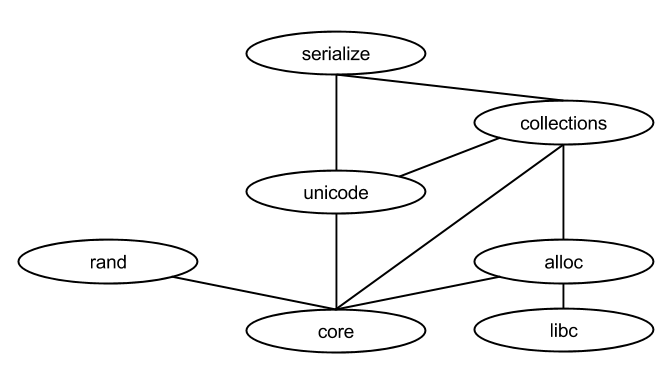
\includegraphics[scale=0.3]{figures/background/rust/embedded-rust-lib.png}
  \end{center}
  \caption{{\rust} Embedded Library}
  \label{fig:rust:rel}
\end{figure}

\subsection{The Core Library}
\label{sec:rust:core}

As described in \autoref{sec:rcl} the \gls{rcl} defines the \emph{core} functionality of the {\rust} language.
These includes the primitive types listed in \autoref{tab:rust:datatypes} in addition to some key datastructures as \code{Option} and \code{Result} as described in \autoref{ssub:rust:features}.
\gls{rcl} defines functionality to work with atomic values and cells along with exposing compiler \concept{intrinsics} which are used for example to provide \concept{volatile} access to memory.
The \gls{rcl} does not have any library dependencies, but in order to use the library without \gls{rsl} a few definitions given in \autoref{tab:core:definitions} must exists.

\begin{table}[H]
  \begin{tabular}{l l}
    \code{memcpy, memcmp, memset} & basic memory management \\
    \code{rust\_begin\_unwind} & handling panicing \\
  \end{tabular}
  \caption{}
  \label{tab:core:definitions}
\end{table}

The memory management functions given in \autoref{tab:core:definitions} are provided by \lib{newlib} and are exposed thought the \lib{startup} library described in \autoref{sec:startup}.
The \code{rust\_begin\_unwind} is also defined in \lib{startup}, but the implementation is only an infinite loop to aid debugging.
In contrast the definition of \code{rust\_begin\_unwind} given in {\std} will abort the program and print an error message.

\subsection{The Allocation Library}
\label{sec:rust:allocation}

Heap allocation is introduced in a library called \lib{alloc}.
The library defines the owned pointer \code{Box} which is {\rust}'s main means of allocating memory on the heap.
In addition the allocation library defines the types \code{Rc} and \code{Arc} which are {\rust}'s reference counted and atomically reference counted heap pointers.
The allocation library is by default dependent on \lib{libc}, but by suppling the \flag{--cfg feature="external\_funcs"} this dependency can be broken.
When breaking this dependency the allocation library requires the functions in \autoref{tab:alloc:external-funcs} to be defined.

\begin{listing}[H]
  \begin{minted}{rust}
rust_allocate(usize, usize) -> *mut u8;
rust_deallocate(*mut u8, usize, usize);
rust_reallocate(*mut u8, usize, usize, usize) -> *mut u8;
  \end{minted}
  \caption{External Dependencies of Allocation Library}
  \label{tab:alloc:external-funcs}
\end{listing}

\subsection{The Collection Library}

The {\rust} collection library provides general purpose data structures.
Of which the \code{Vector} and the \code{String} are the most notable, described below.
As one would guess the collection library depends on the allocation library as it needs to allocate memory on the heap.
The \lib{unicode} dependency is due to the \code{String} type is defined as a valid UTF-8 string.

\subsubsection{Vector}

The Vector is an important data structure both in direct usage but also as a building block for other data structures.
In essence it is a growable heap allocated list of values of the same type.

\subsubsection{String}

The \code{String} defined in the collection library is a owned heap allocated mutable string.
This type is in contrast to the primitive \code{str} type implemented in \gls{rcl}.
